\documentclass[]{article}

% Imported Packages
%------------------------------------------------------------------------------
\usepackage{amssymb}
\usepackage{amstext}
\usepackage{amsthm}
\usepackage{amsmath}
\usepackage{enumerate}
\usepackage{fancyhdr}
\usepackage[margin=1in]{geometry}
\usepackage{graphicx}
\usepackage{extarrows}
\usepackage{setspace}
%------------------------------------------------------------------------------

% Header and Footer
%------------------------------------------------------------------------------
\pagestyle{plain}  
\renewcommand\headrulewidth{0.4pt}                                      
\renewcommand\footrulewidth{0.4pt}                                    
%------------------------------------------------------------------------------

% Title Details
%------------------------------------------------------------------------------
\title{SE 3A04: Software Design II -- Large System Design}
\author{Team 11}
\date{}  
                             
%------------------------------------------------------------------------------

% Document
%------------------------------------------------------------------------------

\begin{document}

\maketitle
\begin{center}
\hrule
	\vspace{0.2in}
\huge AudioVal.ly
	\vspace{0.05in}
\hrule
	\vspace{0.2in}
\huge  Deliverable 2 - High-Level Architectural Design
	\vspace{0.2in}

\large March 9, 2018
\\
	\vspace{1in}
			\large Team 11
\end{center}
\begin{minipage}[c]{\linewidth}
%\fontsize{14pt}{25pt}\selectfont
			\large
			\centering
			\begin{tabular}{l c c}
				Baltej Toor & 1413818 & toorbs \\
				Brandon Roberts & 400018117 & roberb1 \\
				Corey Szeto & 400025728 & szetoc \\
				Jiahong Dong & 1452923 & dongjh \\
				Puru Jetly & 1417837 & jetlyp \\
			\end{tabular}
\end{minipage}	
\newpage

\tableofcontents
\newpage
\section{Introduction}
\label{sec:introduction}
% Begin Section

This section outlines the purpose and provides a system description of the AudioVal.ly project; along with an overview of the contents and organization of this high-level architectural design document.
 


\subsection{Purpose}
\label{sub:purpose}
% Begin SubSection
The purpose of this document to define the use cases, layout the Analysis Class Diagram, describe the Architectural Design, and finally document the class responsibilities through collaboration cards. This document builds on top of and extends the Software Requirements Specification document in that this document describes the way in which the system will interact with the outside world and how the subsystems will be architecturally and logically arranged. \\
The target audience for this document are the stakeholders (Dr. Ridha Khedri, Spencer Deevy and Andrew Le Clair), and any current or future architects, designers and developers of this project.
% End SubSection

\subsection{System Description}
\label{sub:system_description}
% Begin SubSection
The AudioVal.ly application is intended to be a means to identify different genres of music.
The primary interface between the user and the software system is through a device running the Android operating system. This document defines the way in which the users will be expected to interact with the system and how the application will be decomposed into smaller subsystems to reduce the complexity and improve the maintainability, flexibility of this system.

Specifically, the users of this system (application) are expected to perform a set of events that will prompt the system to react. The decomposition will then show how the subsystems will communicate among one another in order to efficiently distribute the work and perform the required actions in response to the user's actions.

% End SubSection

\subsection{Overview}
\label{sub:overview}
% Begin SubSection
The remainder of the document is organized into 4 sections: Use Case Diagram -- how the users and system will interact, Analysis Class Diagram -- the subsystems that compose this entire application, Architectural Design -- the layout of the subsystems into a well-understood software architecture, and Class responsibility collaboration Cards -- description of the interactions between the subsystems. Each section uses an appropriate notation and diagrams
to document the design decision and describe the details of the high-level design of this system.

% End SubSection

% End Section
\newpage
\section{Use Case Diagram}
\label{sec:use_case_diagram}
% Begin Section
\begin{center}
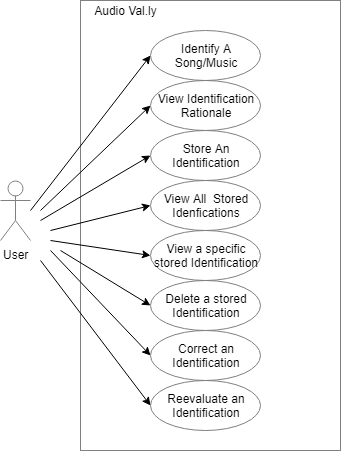
\includegraphics[scale=0.75]{uc}
\end{center}
This use case diagram describes the many business events that can take place for the user.
% End Section

\newpage
\section{Analysis Class Diagram}
\label{sec:analysis_class_diagram}
% Begin Section
The following is an analysis class diagram for the AudioVal.ly application.
\begin{center}
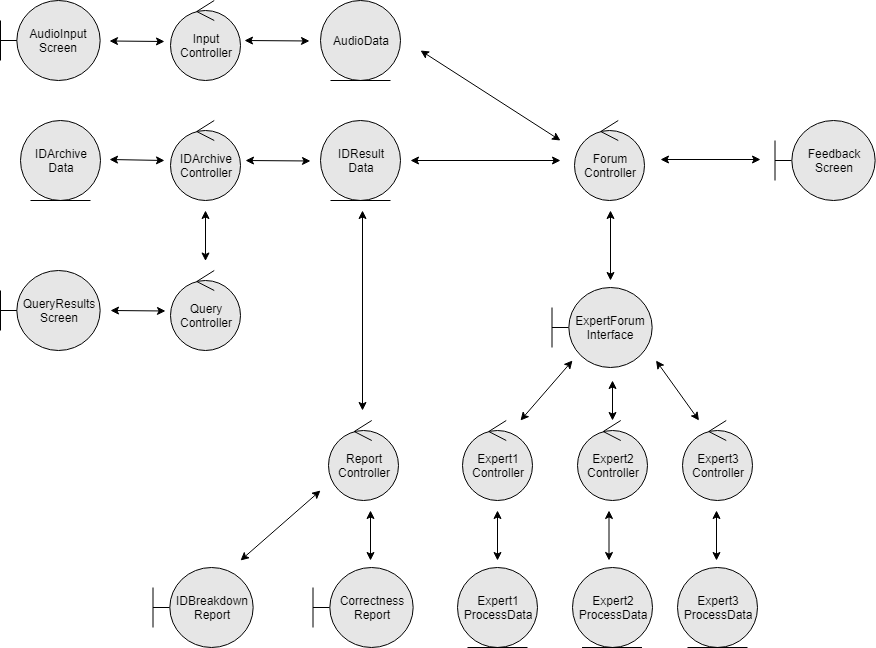
\includegraphics[scale=0.5]{analysisclass}
\end{center}
% End Section

\newpage
\section{Architectural Design}
\label{sec:architectural_design}
% Begin Section
This section provides an overview of the overall architectural design of AudioVal.ly.

\subsection{System Architecture}
\label{sub:system_architecture}
% Begin SubSection
The blackboard architecture design pattern was used when designing the system. The system consists of five major subsystems which are: 
\begin{itemize}
\item Input
\item Forum-Experts
\item Minor subsystems:
\begin{itemize}
\item Reporting
\item Archiving/History
\item Querying 
\end{itemize}
\end{itemize}
The blackboard architecture design pattern is used in situations where there is no known algorithmic solution strategy to solve a problem. Several specialized subsystems will gather information, and a central forum will build a partial or approximate solution to the problem. \\
In the case of this system, since there is not a algorithmic way to identify the genre of the music it is logical to construct a partial understanding of the genre. In the system, three experts each have their own specialized knowledge. Each expert works independently to process information from the forum and generate useful information and a determination. Each expert will provide a piece of information according to their limited knowledge and the forum aggregates the information to a reach an approximate final solution to be stored in the datastore. The input to forum-experts subsystems represent the core of the system's blackboard architecture. The minor subsystems of reporting, archiving/history and querying interact with the core architecture elements to deliver additional functionality without affecting the main architecture design of the system.
% End SubSection

\subsection{Subsystems}
\label{sub:subsystems}
% Begin SubSection
\textbf{Input} The input subsystem provides an interface for the user to record raw audio (music) which is sent as audio input for identification. The subsystem also controls and coordinates validation and storage of the data. It interfaces with the forum-experts subsystem to supply the initial input to be partitioned. \\
\textbf{Forum-Experts} The forum-experts subsystem consists of a central forum (blackboard) that initially distributes data to the three individual experts (each with distinct knowledge set). Each expert analyses the audio data input based on their respective knowledge base to reach a partial solution/identification. These partial solutions/identifications are sent to and aggregated by the forum which resolves any conflicts and communicates feedback updates to the experts for processing as required. The forum sends resulting identification to the archiving (history) subsystem and interacts with the reporting subsystem (through resulting data) to generate user reports based on the overall solution. \\
\textbf{Reporting} The reporting subsystem handles report generation based on forum-expert identification processing for the user. It interacts with the forum-experts subsystem (through resulting data) for identification breakdown and correction reporting. \\
\textbf{Archiving/History} The archiving/history subsystem handles storage and access of past identification result data. The subsystem receives information from the forum-expert subsystem and interacts with the querying subsystem to coordinate access and querying of stored data.\\
\textbf{Querying} The querying subsystem handles data querying/access for past identification result data. The subsystem interacts with the archiving/history subsystem to perform this function.\\
% End SubSection

% End Section

\newpage	
\section{Class Responsibility Collaboration (CRC) Cards}
\label{sec:class_responsibility_collaboration_crc_cards}
% Begin Section

	
	\begin{table}[ht]
		\centering
		\begin{tabular}{|p{5cm}|p{5cm}|}
		\hline 
		 \multicolumn{2}{|l|}{\textbf{Class Name: AudioInputScreen}} \\
		\hline
		\textbf{Responsibility:} & \textbf{Collaborators:} \\
		\hline
		Allow user to input audio for identification &  \\
		\hline
		Receive audio information from the device microphone &  \\
		\hline
		Display input validation errors &  \\
		\hline
		Receive request to take audio input & InputController \\
		\hline
		\end{tabular}
	\end{table}
	
	\begin{table}[ht]
		\centering
		\begin{tabular}{|p{5cm}|p{5cm}|}
		\hline 
		 \multicolumn{2}{|l|}{\textbf{Class Name: InputController}} \\
		\hline
		\textbf{Responsibility:} & \textbf{Collaborators:} \\
		\hline
		Store valid audio information in audio data storage & AudioInputScreen, \mbox{AudioData} \\
		\hline
		Validate audio input &  \\
		\hline
		Request audio input & AudioInputScreen \\
		\hline
		\end{tabular}
	\end{table}
	
	\begin{table}[ht]
		\centering
		\begin{tabular}{|p{5cm}|p{5cm}|}
		\hline 
		 \multicolumn{2}{|l|}{\textbf{Class Name: AudioData}} \\
		\hline
		\textbf{Responsibility:} & \textbf{Collaborators:} \\
		\hline
		Represent validated audio information inputted by user & \\
		\hline
		\end{tabular}
	\end{table}
	
\newpage
	\begin{table}[ht]
		\centering
		\begin{tabular}{|p{5cm}|p{5cm}|}
		\hline 
		 \multicolumn{2}{|l|}{\textbf{Class Name: ForumController}} \\
		\hline
		\textbf{Responsibility:} & \textbf{Collaborators:} \\
		\hline
		Distribute stored audio data to Expert(s) for processing & AudioData \mbox{ExpertForumInterface} \\
		\hline
		Receive Expert(s) identification results & ExpertForumInterface \\
		\hline
		Resolve conflict between conflicting Expert identifications & \\
		\hline
		Store identification result report to identification storage & IDResultData \\
		\hline
		Send feedback/update information to Expert(s) & ExpertForumInterface \mbox{FeedbackScreen} \\
		\hline
		Send overall identification result to FeedbackScreen & FeedbackScreen \\
		\hline
		Prompt FeedbackScreen to display result & FeedbackScreen \\
		\hline
		Receive correctness data/result correction for the identification & FeedbackScreen \\
		\hline
		Store correction data to identification storage & IDResultData \\
		\hline
		\end{tabular}
	\end{table}
	
	\begin{table}[ht]
		\centering
		\begin{tabular}{|p{5cm}|p{5cm}|}
		\hline 
		 \multicolumn{2}{|l|}{\textbf{Class Name: FeedbackScreen}} \\
		\hline
		\textbf{Responsibility:} & \textbf{Collaborators:} \\
		\hline
		Receive identification result & ForumController \\
		\hline
		Display identification result &  \\
		\hline
		Allow user to provide correctness feedback on result &  \\
		\hline
		Receive correctness feedback from user &  \\
		\hline
		Compare user correction to determined identification result &  \\
		\hline
		Send individual Expert correctness data/result correction for the identification to Forum to store & ForumController \\
		\hline
		\end{tabular}
	\end{table}
	
\newpage
	\begin{table}[ht]
		\centering
		\begin{tabular}{|p{5cm}|p{5cm}|}
		\hline 
		 \multicolumn{2}{|l|}{\textbf{Class Name: ExpertForumInterface}} \\
		\hline
		\textbf{Responsibility:} & \textbf{Collaborators:} \\
		\hline
		Pass initial audio data from Forum and Expert(s) & ForumController \mbox{Expert1Controller} \mbox{Expert2Controller} \mbox{Expert3Controller} \\
		\hline
		Pass identification result(s) from Expert(s) to Forum & ForumController \mbox{Expert1Controller} \mbox{Expert2Controller} \mbox{Expert3Controller} \\
		\hline
		Transfer updates between Forum and Expert(s) & ForumController \mbox{Expert1Controller} \mbox{Expert2Controller} \mbox{Expert3Controller} \\
		\hline
		\end{tabular}
	\end{table}
	
	\begin{table}[ht]
		\centering
		\begin{tabular}{|p{5cm}|p{5cm}|}
		\hline 
		 \multicolumn{2}{|l|}{\textbf{Class Name: Expert1Controller}} \\
		\hline
		\textbf{Responsibility:} & \textbf{Collaborators:} \\
		\hline
		Receive audio data & ExpertForumInterface \\
		\hline
		Process audio data based on specified computation criteria &  \\
		\hline
		Store information in ProcessData & Expert1ProcessData \\
		\hline
		Determine identification result based on processing &  \\
		\hline
		Send identification result to Forum & ExpertForumInterface \\
		\hline
		Receive information (updates) from Forum & ExpertForumInterface \\
		\hline
		Utilize ProcessData for identification & Expert1ProcessData \\
		\hline
		\end{tabular}
	\end{table}
	
\newpage
	\begin{table}[ht]
		\centering
		\begin{tabular}{|p{5cm}|p{5cm}|}
		\hline 
		 \multicolumn{2}{|l|}{\textbf{Class Name: Expert2Controller}} \\
		\hline
		\textbf{Responsibility:} & \textbf{Collaborators:} \\
		\hline
		Receive audio data & ExpertForumInterface \\
		\hline
		Process audio data based on specified computation criteria &  \\
		\hline
		Store information in ProcessData & Expert2ProcessData \\
		\hline
		Determine identification result based on processing &  \\
		\hline
		Send identification result to Forum & ExpertForumInterface \\
		\hline
		Receive information (updates) from Forum & ExpertForumInterface \\
		\hline
		Utilize ProcessData for identification & Expert2ProcessData \\
		\hline
		\end{tabular}
	\end{table}

	\begin{table}[ht]
		\centering
		\begin{tabular}{|p{5cm}|p{5cm}|}
		\hline 
		 \multicolumn{2}{|l|}{\textbf{Class Name: Expert3Controller}} \\
		\hline
		\textbf{Responsibility:} & \textbf{Collaborators:} \\
		\hline
		Receive audio data & ExpertForumInterface \\
		\hline
		Process audio data based on specified computation criteria &  \\
		\hline
		Store information in ProcessData & Expert3ProcessData \\
		\hline
		Determine identification result based on processing &  \\
		\hline
		Send identification result to Forum & ExpertForumInterface \\
		\hline
		Receive information (updates) from Forum & ExpertForumInterface \\
		\hline
		Utilize ProcessData for identification & Expert3ProcessData \\
		\hline
		\end{tabular}
	\end{table}	
	
	\begin{table}[ht]
		\centering
		\begin{tabular}{|p{5cm}|p{5cm}|}
		\hline 
		 \multicolumn{2}{|l|}{\textbf{Class Name: Expert1ProcessData}} \\
		\hline
		\textbf{Responsibility:} & \textbf{Collaborators:} \\
		\hline
		Represent Expert 1 processing information/data &  \\
		\hline
		Allow updates from Expert 1 & Expert1Controller \\
		\hline
		Represent identification result for the Expert 1 &  \\
		\hline
		\end{tabular}
	\end{table}
	
\newpage
	\begin{table}[ht]
		\centering
		\begin{tabular}{|p{5cm}|p{5cm}|}
		\hline 
		 \multicolumn{2}{|l|}{\textbf{Class Name: Expert2ProcessData}} \\
		\hline
		\textbf{Responsibility:} & \textbf{Collaborators:} \\
		\hline
		Represent Expert 2 processing information/data &  \\
		\hline
		Allow updates from Expert 2 & Expert2Controller \\
		\hline
		Represent identification result for the Expert 2 &  \\
		\hline
		\end{tabular}
	\end{table}
	
	\begin{table}[ht]
		\centering
		\begin{tabular}{|p{5cm}|p{5cm}|}
		\hline 
		 \multicolumn{2}{|l|}{\textbf{Class Name: Expert3ProcessData}} \\
		\hline
		\textbf{Responsibility:} & \textbf{Collaborators:} \\
		\hline
		Represent Expert 3 processing information/data &  \\
		\hline
		Allow updates from Expert 3 & Expert3Controller \\
		\hline
		Represent identification result for the Expert 3 &  \\
		\hline
		\end{tabular}
	\end{table}
	
	\begin{table}[ht]
		\centering
		\begin{tabular}{|p{5cm}|p{5cm}|}
		\hline 
		 \multicolumn{2}{|l|}{\textbf{Class Name: IDResultData}} \\
		\hline
		\textbf{Responsibility:} & \textbf{Collaborators:} \\
		\hline
		Represent identification result data &  \\
		\hline
		Allow updates by Forum &  ForumController \\
		\hline
		\end{tabular}
	\end{table}
	
\newpage
	\begin{table}[ht]
		\centering
		\begin{tabular}{|p{5cm}|p{5cm}|}
		\hline 
		 \multicolumn{2}{|l|}{\textbf{Class Name: IDArchiveController}} \\
		\hline
		\textbf{Responsibility:} & \textbf{Collaborators:} \\
		\hline
		Retrieve identification result information & IDResultData \\
		\hline
		Archive identification result information & IDArchiveData \\
		\hline
		Receive query on identification archive & QueryController \\
		\hline
		Perform query on identification archive &  \\
		\hline
		Return query result & QueryController \\
		\hline
		Receive deletion request of archive data & QueryController \\
		\hline
		Delete specified archive data &  \\
		\hline
		\end{tabular}
	\end{table}
	

	\begin{table}[ht]
		\centering
		\begin{tabular}{|p{5cm}|p{5cm}|}
		\hline 
		 \multicolumn{2}{|l|}{\textbf{Class Name: IDArchiveData}} \\
		\hline
		\textbf{Responsibility:} & \textbf{Collaborators:} \\
		\hline
		Represent historical identification result(s) data &  \\
		\hline
		\end{tabular}
	\end{table}
	
	\begin{table}[ht]
		\centering
		\begin{tabular}{|p{5cm}|p{5cm}|}
		\hline 
		 \multicolumn{2}{|l|}{\textbf{Class Name: QueryController}} \\
		\hline
		\textbf{Responsibility:} & \textbf{Collaborators:} \\
		\hline
		Request query on archived identification data & IDArchiveController \\
		\hline
		Receive query result & IDArchiveController \\
		\hline
		Prompt ResultsScreen to display query result & QueryResultsScreen \\
		\hline
		Request archive data deletion & IDArchiveController \\
		\hline
		Display deletion confirmation &  \\
		\hline
		\end{tabular}
	\end{table}
	
\newpage
	\begin{table}[ht]
		\centering
		\begin{tabular}{|p{5cm}|p{5cm}|}
		\hline 
		 \multicolumn{2}{|l|}{\textbf{Class Name: QueryResultsScreen}} \\
		\hline
		\textbf{Responsibility:} & \textbf{Collaborators:} \\
		\hline
		Receive query result on identification archive & QueryController \\
		\hline
		Display query result to user &  \\
		\hline
		Display archived identification data &  \\
		\hline
		Respond to Delete result record from archive & QueryController \\
		\hline
		\end{tabular}
	\end{table}
	
	\begin{table}[ht]
		\centering
		\begin{tabular}{|p{5cm}|p{5cm}|}
		\hline 
		 \multicolumn{2}{|l|}{\textbf{Class Name: ReportController}} \\
		\hline
		\textbf{Responsibility:} & \textbf{Collaborators:} \\
		\hline
		Receive information on recent identification result and processing & IDResultData \\
		\hline
		Generate report based on specified criteria &  \\
		\hline
		Prompt corresponding screen to display report & IDBreakdownReport \mbox{CorrectnessReport} \\
		\hline
		\end{tabular}
	\end{table}
	
	\begin{table}[ht]
		\centering
		\begin{tabular}{|p{5cm}|p{5cm}|}
		\hline 
		 \multicolumn{2}{|l|}{\textbf{Class Name: IDBreakdownReport}} \\
		\hline
		\textbf{Responsibility:} & \textbf{Collaborators:} \\
		\hline
		Receive display request for identification breakdown report & ReportController \\
		\hline
		Display identification breakdown report &  \\
		\hline
		\end{tabular}
	\end{table}
	
\newpage
	\begin{table}[ht]
		\centering
		\begin{tabular}{|p{5cm}|p{5cm}|}
		\hline 
		 \multicolumn{2}{|l|}{\textbf{Class Name: CorrectnessReport}} \\
		\hline
		\textbf{Responsibility:} & \textbf{Collaborators:} \\
		\hline
		Receive display request for correctness report & ReportController \\
		\hline
		Display identification correctness report &  \\
		\hline
		\end{tabular}
	\end{table}
	
\newpage
%\end{enumerate}
% End Section
\newpage
\appendix
\section{Division of Labour}
\label{sec:division_of_labour}
\begin{center}
\large
			\begin{tabular}{l|c}
				Work Completed   & Contributors \\\hline
				Production Conceptualisation &Team 11 \\
				HLAD Section 1 : Introduction & Puru Jetly \\
				HLAD Section 2 : Use Case Diagram  & Brandon Roberts, Corey Szeto \\
				HLAD Section 3 : Analysis Class Diagram  & Baltej Toor  \\
				HLAD Section 4 : Architectural Design  & Jiahong Dong \\
				HLAD Final Review + Latex  & Brandon Roberts, Baltej Toor \\
			\end{tabular}
			\vspace{0.1in}
\huge Signatures
\end{center}
			\vspace{0.3in}
\large
			\begin{tabular}{l|r}
			\vspace{1in}
				Baltej Toor  & \underline{\hspace{8cm}} \\
			\vspace{1in}
				Brandon Roberts   & \underline{\hspace{8cm}} \\
			\vspace{1in}
				Corey Szeto  & \underline{\hspace{8cm}} \\
			\vspace{1in}
				Jiahong Dong   & \underline{\hspace{8cm}} \\
			\vspace{1in}
				Puru Jetly   & \underline{\hspace{8cm}} \\
			\end{tabular}

\end{document}
%------------------------------------------------------------------------------